\documentclass[12pt,a4paper,openright,twoside]{book}
\usepackage[utf8]{inputenc}
\usepackage{disi-thesis}
\usepackage{code-lstlistings}
\usepackage{float}
\usepackage{notes}
\usepackage{shortcuts}
\usepackage{acronym}
\usepackage{hyperref} % links
\usepackage{comment} % for multi-line comments
\usepackage{booktabs} % for better tables
\usepackage{xcolor}
\usepackage{listings}
\usepackage{caption}
\usepackage{subcaption}
\usepackage{svg}

\showboxdepth=5
\showboxbreadth=5

\school{\unibo}
\programme{Corso di Laurea Magistrale in Ingegneria e Scienze Informatiche}
\title{Development of an open benchmarking platform for Collective Adaptive Systems}
\author{Paolo Penazzi}
\date{\today}
\subject{Laboratorio di Sistemi Software}
\supervisor{Prof. Danilo Pianini}
\cosupervisor{Prof. Lukas Esterle}
\session{III}
\academicyear{2022-2023}

% Definition of acronyms
\acrodef{CAS}{Collective Adaptive Systems}
\acrodef{vm}[VM]{Virtual Machine}
\acrodef{SUT}{System Under Test}


\mainlinespacing{1.241} % line spacing in main matter, comment to default (1)

\begin{document}

\frontmatter\frontispiece

\begin{abstract}
  Max 2000 characters, strict.
\end{abstract}

%----------------------------------------------------------------------------------------
\tableofcontents
\listoffigures     % (optional) comment if empty
\lstlistoflistings % (optional) comment if empty
%----------------------------------------------------------------------------------------

\mainmatter

%----------------------------------------------------------------------------------------
\chapter{Introduction}
\label{chap:introduction}
%----------------------------------------------------------------------------------------
\paragraph{Background and Motivation}
One aspect that guides scientific research is the discovery of new solutions that improve what is defined as the state of the art. 

This implies that at some point, it is necessary to compare two solutions and have a clear metric to understand which solution performs better. 
Another fundamental aspect is to have a standard test protocol to compare two algorithms on the same problem, under the same conditions, with the possibility of reproducing experiments. 

In many aspects of computer science, the reproducibility of scientific publications is questioned \cite{DBLP:journals/cacm/CollbergP16, DBLP:conf/aaai/GundersenK18}, which makes the creation of a benchmarking and testing framework necessary. 
In some application domains, such as security \cite{DBLP:conf/bdet/Es-SamaaliOBMK21}, IoT \cite{DBLP:conf/IEEEares/RuckGWLN23} and many more, \cite{DBLP:journals/ral/CollinsRYSJP24, DBLP:journals/corr/abs-2401-01275} tools have been developed for benchmarking. 
In other fields, like autonomic, organic computing, and collective adaptive systems, such frameworks have not yet been created. \cite{DBLP:conf/icac/BrownHHLLSY04, DBLP:conf/autonomics/EtcheversCV09}

\paragraph{Objectives}

This thesis aims to partially fill this gap by creating a benchmarking platform \cite{DBLP:conf/cisis/VilenicaL12, DBLP:conf/atal/ZhangZWBR20} for a specific type of distributed systems: collective adaptive systems. \cite{DBLP:journals/sttt/NicolaJW20}
These systems are characterized by their ability to adapt to the environment in which they are immersed and interact with it. \cite{DBLP:conf/birthday/BucchiaroneM19}
There is no central entity, either internal or external, that coordinates the devices in the network; instead, they collaborate with each other to achieve a goal.
The properties and behavior of these systems make them particularly challenging to test and evaluate their performance. \cite{DBLP:conf/srds/AlmeidaMV10}
This work aims to create a framework to make it easy for the user to define a benchmark and execute it,
allowing him or others to develop new solutions related to a specific problem and compare them with existing ones.
The key to this framework is its extensibility: given the numerous aspects a user might want to evaluate,
the framework must be designed so that adding new simulators is possible without compromising the functionality of already supported simulators. \cite{DBLP:conf/mascots/Dujmovic99}

%----------------------------------------------------------------------------------------
\chapter{Background}
%----------------------------------------------------------------------------------------

\section{Collective Adaptive Systems}

\ac{CAS} are a complex type of distributed network, composed of a large number of heterogeneous entities.
The two main characteristics that distinguish these systems are the ability to adapt their behavior to dynamically changing open-ended environments
and the pursuit of a collective goal, achieved through interaction without specific external or internal central control. \cite{DBLP:series/lncs/HolzlRW08, DBLP:journals/corr/abs-1108-5643}
It is important to note that \ac{CAS} can be composed of heterogeneous entities, each with its capabilities and goals.
To achieve the collective goal without central control, \ac{CAS} often adopts cooperative operating strategies to run distributed decision-making mechanisms. \cite{DBLP:journals/tomacs/Aldini18} \\

Nowadays, many systems are adaptive and collective: drone swarms tasked with monitoring an area,
wearable devices to manage crowd congestion during a public event, cars on streets connected to handle traffic,
are all examples of CAS. \cite{DBLP:journals/sttt/NicolaJW20}

\begin{figure*}[h]
  \centering
  \begin{subfigure}[b]{0.49\textwidth}
    \centering
    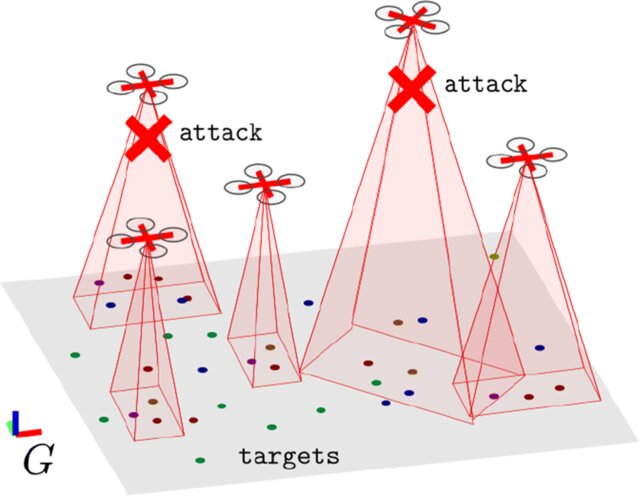
\includegraphics[width=0.9\textwidth]{figures/swarm2.jpeg}
  \end{subfigure}

  \begin{subfigure}[b]{0.49\textwidth}
    \centering
    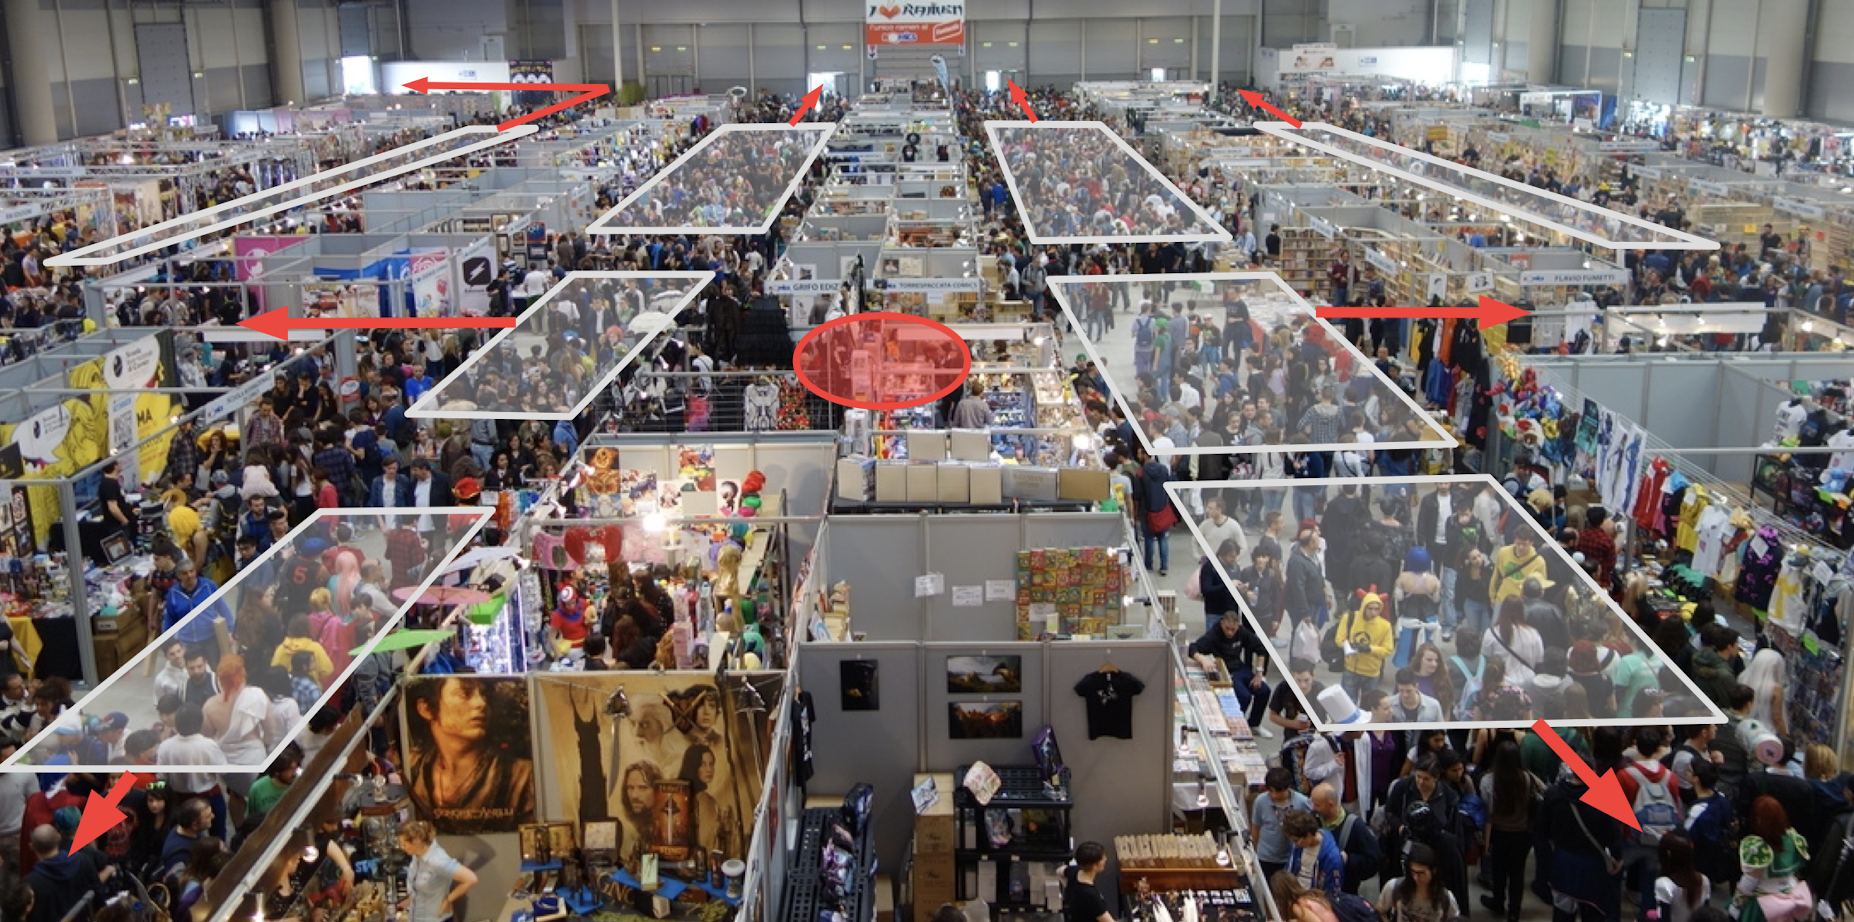
\includegraphics[width=0.8\textwidth]{figures/crowd.png}
  \end{subfigure}
  \caption{Some examples of CAS.}
\end{figure*}

\section{Aggregate Programming}

In recent years, we have witnessed a shift in the production of computing devices: moving from a few large and powerful devices to a large number of small and lightweight devices.
There is often talk about the Internet of Things and how technology has become pervasive, impacting every aspect of our lives with electronic devices.
This trend has led to a change in the way we compute data: no longer focusing on a single machine performing heavy computation, but rather on a distributed network of devices communicating and collaborating to achieve a result.
Computation is thus divided and distributed across various devices in the network.

This has introduced an additional level of complexity in programming these systems as it is necessary to consider issues such as communication between devices,
concurrency, or failures. Furthermore, as these systems grow in complexity, it becomes challenging to create solutions that are extensible, modular, and easily testable. \cite{DBLP:conf/ecoop/CasadeiV16}

Aggregate programming is a new approach to developing complex distributed systems that abstract from individual devices, focusing on programming the collective.
Through a layer that handles and hides some problematic aspects of these networks, such as communication between devices and details of individual entities,
it is possible to simplify the design and maintenance of these systems. \cite{DBLP:journals/computer/BealPV15, DBLP:conf/sfm/BealV16}

Aggregate programming is based on the concept of a computational field, which is a global map associating each device in the network with its local value,
and on that of field calculus, a minimal core that provides basic constructs for working with fields. \cite{DBLP:journals/corr/ViroliADPB16}

\section{Testing}

In every field of engineering, testing is a fundamental part of the development process.
Testing refers to the process carried out to verify and validate a system, according to its requirements. \cite{Spillner2011}
It is important to evaluate the behavior of newly developed algorithms against state-of-the-art solutions.
This allows us to understand whether a newly developed solution is better than an existing one in a certain scenario. \\

The testing of adaptive systems introduces a series of challenges and difficulties, many of which stem from the intrinsic nature of these systems.
Given the complexity of these systems, using a single simulator is not sufficient to test all their features.
It is often necessary to use multiple simulators and combine the results obtained to understand the system's behavior.
This technique is termed co-simulation and introduces various issues, such as communication delays, approximations, and difficulties in synchronizing simulators. \cite{DBLP:journals/simpra/ThuleLGML19}
Since these systems are adaptive and react to changes in their environment, it is natural to want to support the injection of changes. \cite{DBLP:conf/icac/BrownHHLLSY04}
A complete testbed must, therefore, be able to command different existing tools, support various execution environments, and allow the user to test the system in its entirety.

\section{Simulation}

In computer science, simulation is the process of executing software in a controlled environment to evaluate its behavior.
Simulations can be used to test the correctness of a program, evaluate its performance, or understand its behavior in a specific scenario.
The key point of a simulation is to execute the software under controlled and repeatable conditions to compare different executions. \cite{DBLP:journals/cacm/CollbergP16}
This cannot be done without a simulator, which provides the user with all the tools needed to run the simulation. \cite{argun2021simulation, bagrodia1998parsec} \\
The importance of simulators becomes clear when testing \ac{CAS}.
It is not feasible to create a real environment, such as a network of 100 drones or a crowd of 1000 people, to test a program.
Simulators allow us to create a virtual environment where we can run the program and evaluate its behavior. \\

\section{Alchemist}

The reference simulator for this work is Alchemist. \cite{Pianini_2013}
Alchemist is a meta-simulator, open-source, for simulating complex distributed systems. It is termed a meta-simulator because it is based on generic abstractions.
The meta-model of Alchemist is inspired by biochemistry and consists of various entities:
\begin{itemize}
  \item \textbf{Molecule} The name of a data item.
  \item \textbf{Concentration} The value associated with a molecule.
  \item \textbf{Node} A container of molecules and concentrations. Disposed inside the environment.
  \item \textbf{Environment} The abstraction for the space. It contains nodes and can tell the position of a node in the space and the distance between two nodes.
  \item \textbf{Linking Rule} A rule that defines the relation between nodes.
  \item \textbf{Reaction} Events fired according to a time distribution and set of conditions.
  \item \textbf{Condition} A function that takes the current environment as input and outputs a boolean and a number. The output influences the execution of the corresponding reaction.
  \item \textbf{Action} Models a change in the environment.
\end{itemize}

Here is the visual representation of the Alchemist meta-model.

\begin{figure}[h]
  \centering
  \includegraphics[width=\textwidth]{figures/alchemist-model.png}
  \caption{Alchemist meta-model}
\end{figure}

\begin{figure}[h]
  \centering
  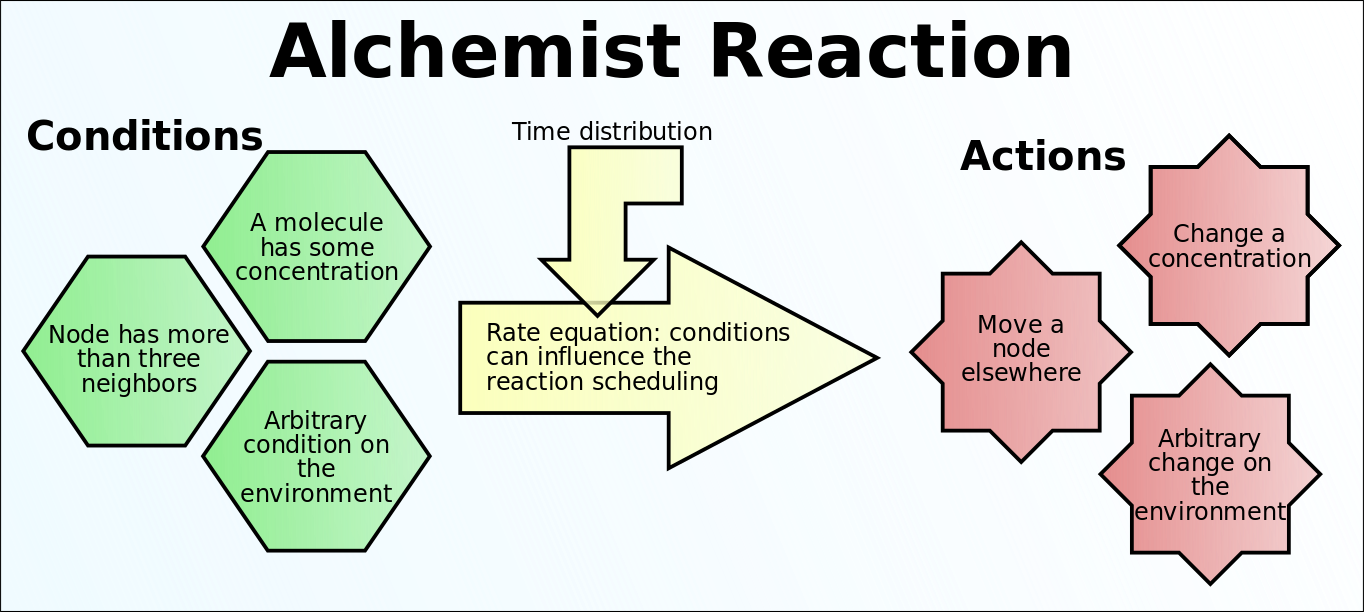
\includegraphics[width=\textwidth]{figures/alchemist-reaction.png}
  \caption{Alchemist reaction}
\end{figure}

The key of the Alchemist extensibility is the very generic interpretation of molecules and concentrations. An incarnation maps this generic chemical abstraction to a specific use case.
Alchemist supports four incarnations:
SAPERE \cite{DBLP:conf/saso/CastelliMRZ11}, the first supported incarnation, based on the concept of Live Semantic Annotation (LSA),
ScaFi \cite{DBLP:journals/softx/CasadeiVAP22}, which is a Scala-based library and framework for Aggregate Programming,
Protelis \cite{DBLP:conf/sac/PianiniVB15}, a programming language for aggregate computing, and
Biochemistry incarnation.

\begin{figure}[h]
  \centering
  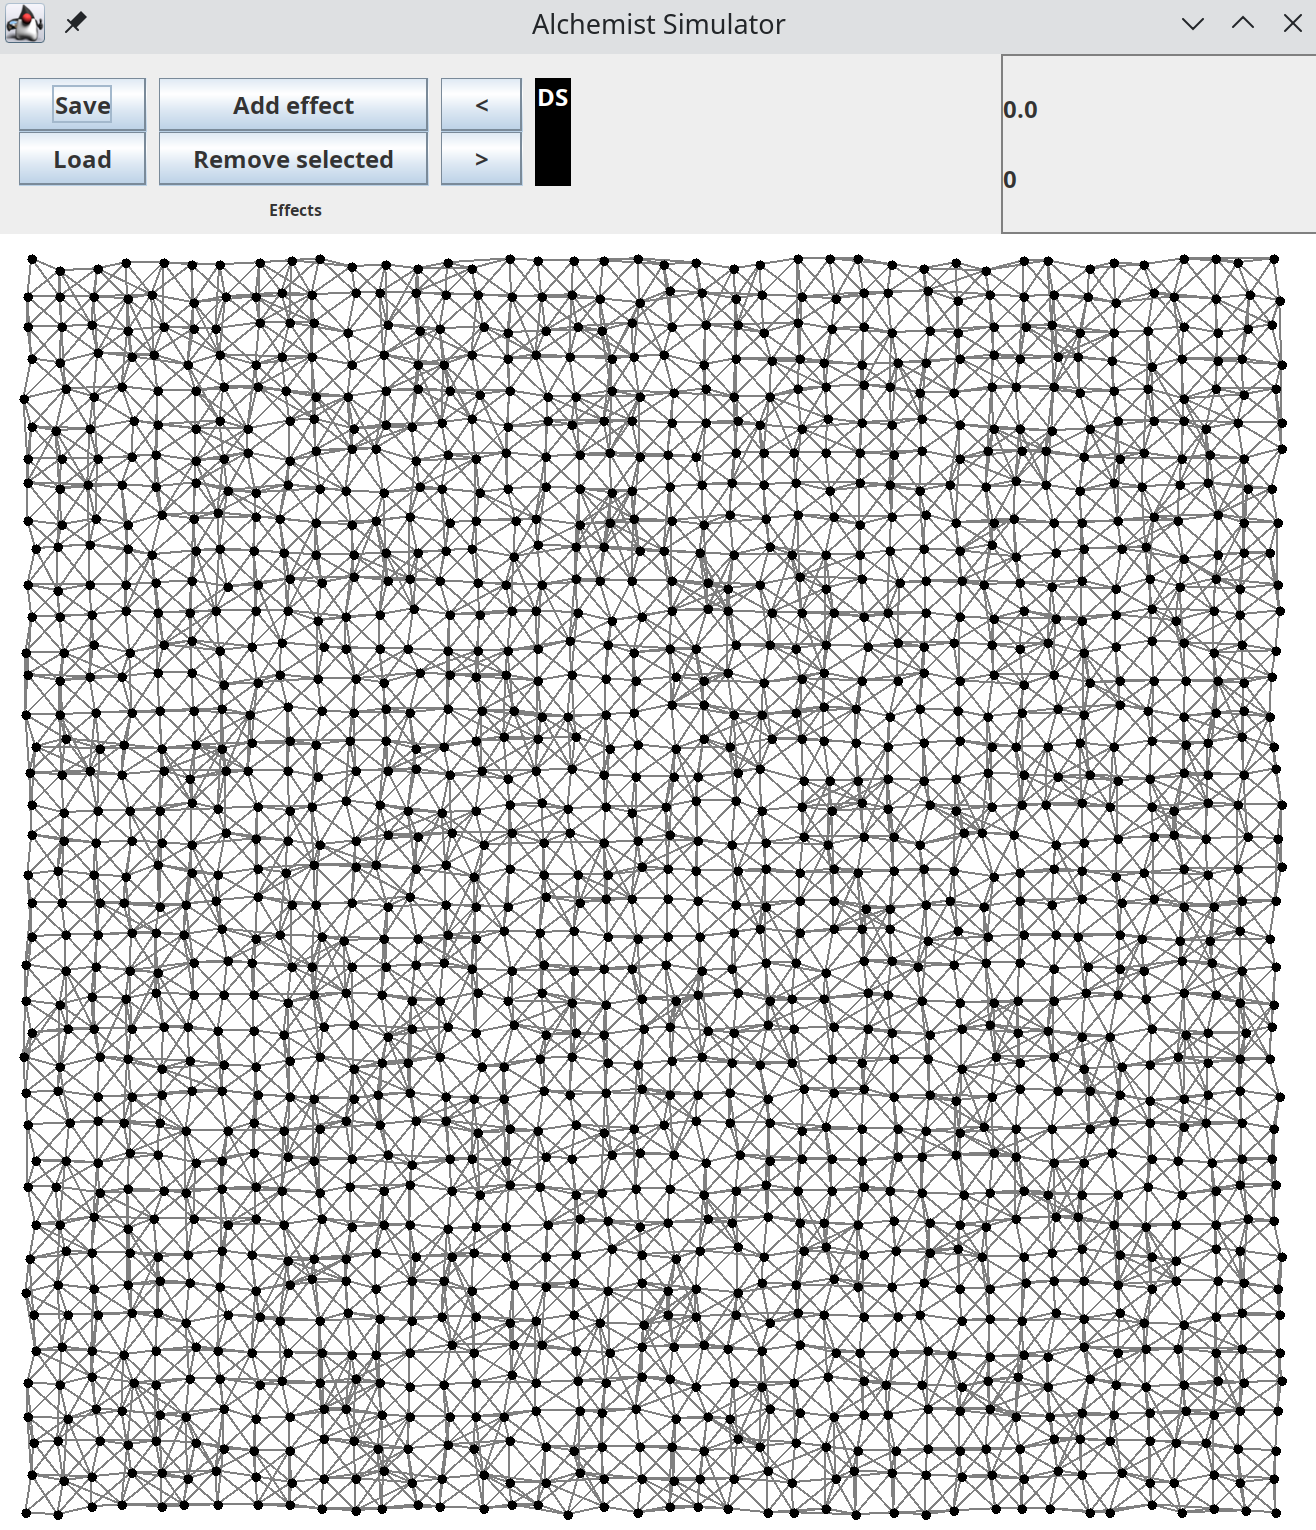
\includegraphics[width=\textwidth]{figures/alchemist.png}
  \caption{A grid of nodes in Alchemist}
\end{figure}

\section{NetLogo}

NetLogo is a programmable modeling environment for simulating natural and social phenomena. It was created at the Center
for Connected Learning and Computer-Based Modeling (CCL) at Northwestern University, directed by Uri Wilensky.

NetLogo is particularly well suited for modeling complex systems developing over time.
Users can program the behavior of thousands of independent agents to see how the system-level behavior emerges from the interactions of the agents.

It also comes with the Models Library, a large collection of pre-written simulations that can be used and modified.
These simulations can be explored to observe their behavior under various conditions.

The following image shows the NetLogo interface while executing one of the bundled simulations.

\begin{figure}[h]
  \centering
  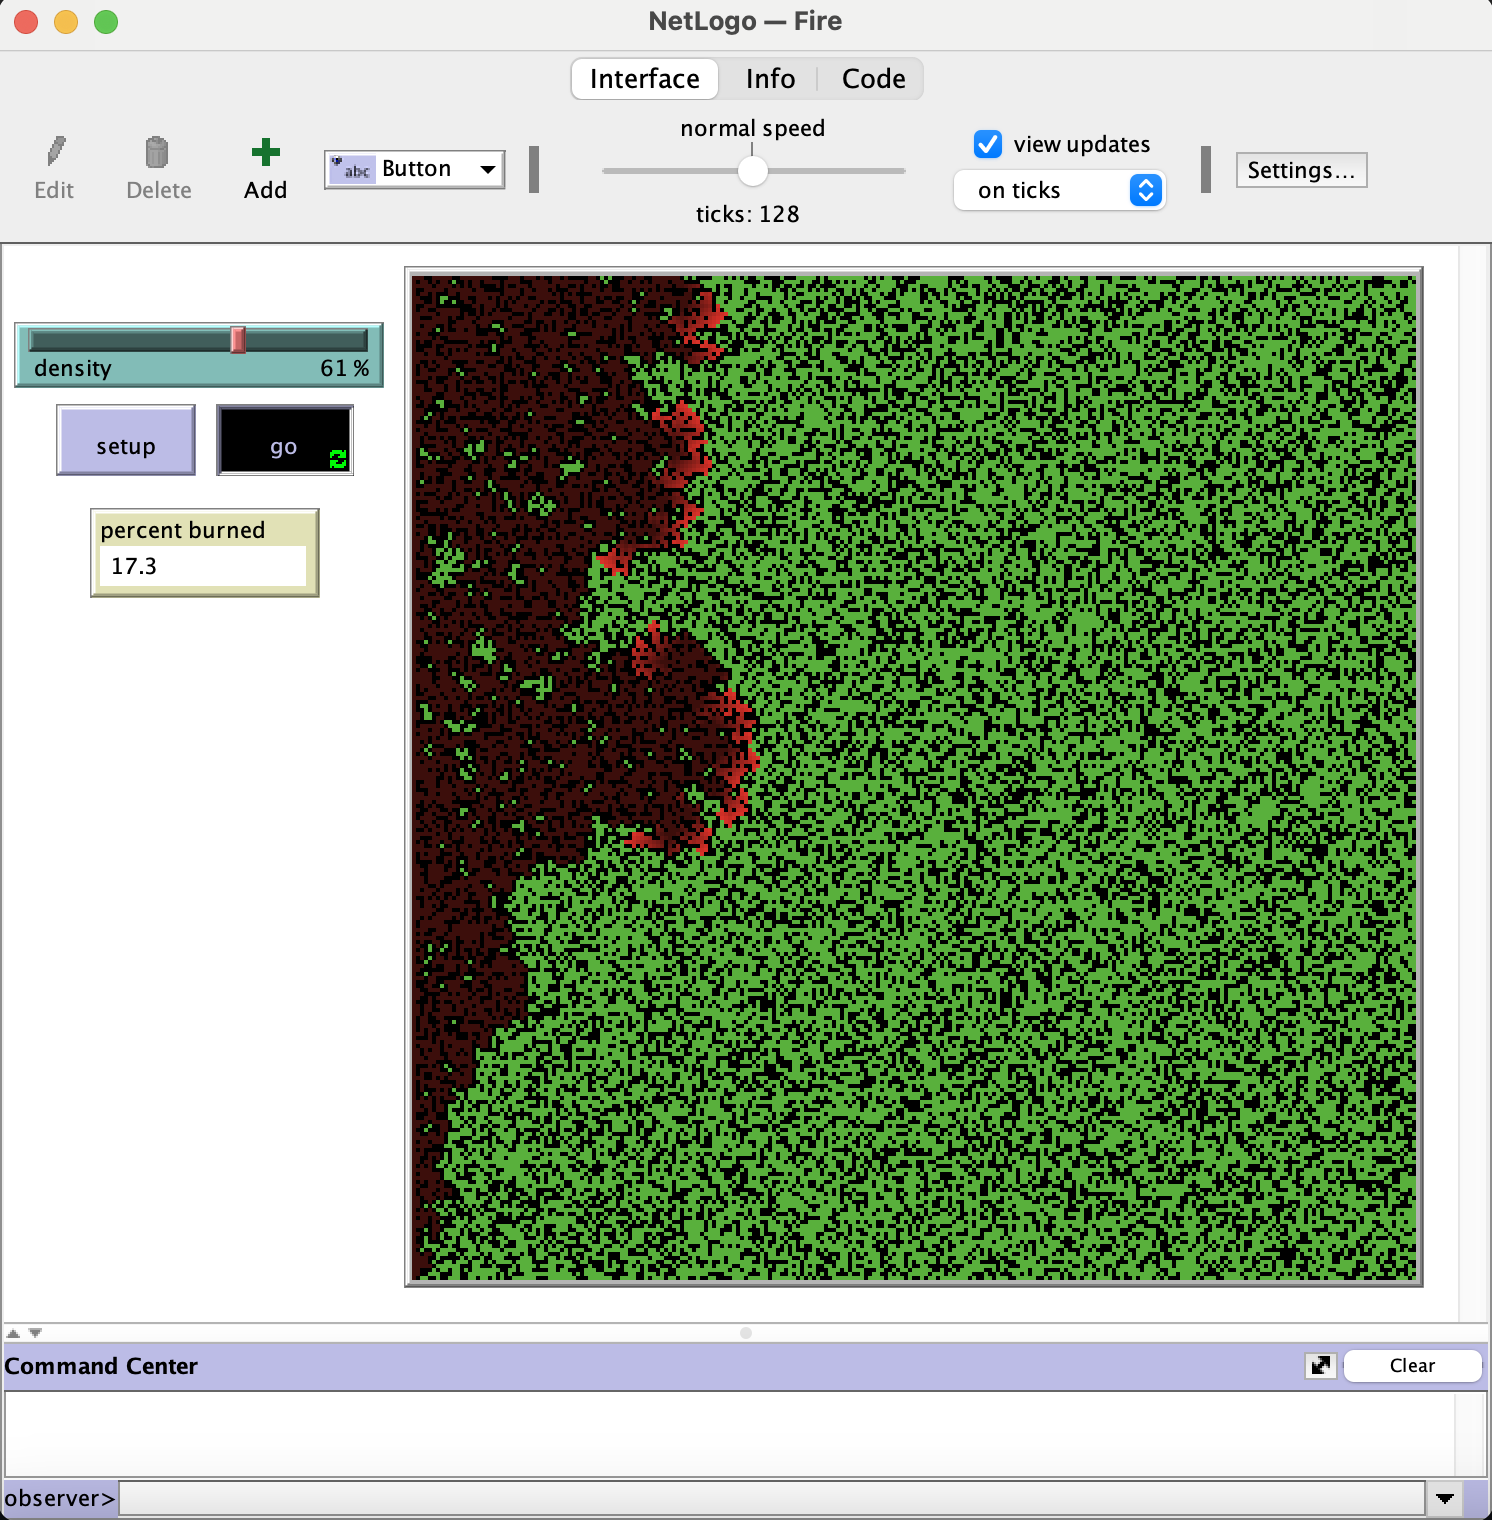
\includegraphics[width=0.8\textwidth]{figures/NetLogo-interface.png}
  \caption{NetLogo interface}
\end{figure}

The model used in the image above is the Fire model.
It simulates the spread of a fire through a forest. It shows that the fire's chance of reaching the right edge
of the forest depends critically on the density of trees.

%----------------------------------------------------------------------------------------
\chapter{Analysis}
%----------------------------------------------------------------------------------------

\section{Domain}

A domain-driven approach was employed in the development. The choices made were based on the study of existing simulators and user needs.

To better understand the problem domain and to avoid misunderstandings, a ubiquitous language has been defined.
These concepts were then utilized in the framework development and can be found in the implementation.

\begin{table}[h]
  \centering
  \begin{tabular}{|l|p{0.8\textwidth}|}
    \toprule
    \textbf{Term} & \textbf{Meaning}                                                                                                                                                                                    \\
    \midrule
    Testing       & The overall process carried out to verify and validate a system, according to requirements, to promote the desired internal and external quality and to mitigate risks in development and products. \\ \hline
    Testbed       & A platform for rigorous, transparent and replicable environment for experimentation and testing                                                                                                     \\ \hline
    Solution      & A set of algorithms leading to achieving goals and overcoming the problem posted                                                                                                                    \\ \hline
    Scenario      & Contains all the information about the test execution: the simulation platform, the metrics, the input parameters                                                                                   \\ \hline
    Simulator     & A software that allows the user to see how its program would behave in a real environment                                                                                                           \\ \hline
  \end{tabular}
  \caption{Domain Ubiquitous Language}
\end{table}

User Stories were also defined, helpful in understanding what users need and thus what features the framework should support.

\begin{table}[h]
  \centering
  \begin{tabular}{|p{0.8\textwidth}|}
    \toprule
    \textbf{User Story}                                                                                   \\
    \midrule
    \textit{...As a user, I want to be able to create a benchmark.}                                       \\ \hline
    \textit{...As a user, I want to be able to use different simulators.}                                 \\ \hline
    \textit{...As a user, I want to be able to define and execute different scenarios.}                   \\ \hline
    \textit{...As a user, I want to be able to define a solution.}                                        \\ \hline
    \textit{...As a user, I want to be able to define how the output of the benchmark will be processed.} \\ \hline
    \textit{...As a user, I want to be able to compare my solution to other's.}                       \\ \hline
  \end{tabular}
  \caption{Domain Ubiquitous Language}
\end{table}

It is important to note that the expected users of the framework are researchers and developers,
who are people with a strong technical background and knowledge of the domain.

\section{Requirements}

\subsection*{User Requirements}
These requirements express the needs of the user and identify which actions the user should be able to perform.
The following requirements are extracted from the previous domain analysis:
\begin{itemize}
  \item It should be possible to define a \emph{benchmark}.
  \item It should be possible to define a \emph{scenario}.
  \item It should be possible to apply a \emph{solution} to an existing scenario.
  \item It should be possible to download and use different \emph{simulators}.
  \item It should be possible to execute a benchmark.
  \item It should be possible to define which \emph{metric} to extract from the benchmark's output.
  \item It should be possible to compare the results of different solutions.
  \item It should be possible to extend the framework to support new simulators.
\end{itemize}

\subsection*{Functional Requirements}
Functional requirements define what are the features and functions of the framework.
These are derived from the user requirements.

\begin{itemize}
  \item The framework should allow the user to define a benchmark.
  \item The framework should allow the user to define a scenario.
  \item The framework should allow the user to run a scenario with any solution.
  \item The framework should allow the user to use different simulators, providing a way to download them.
  \item The framework should allow the user to execute a benchmark.
  \item The framework should allow the user to define which metric to extract from the benchmark's output.
  \item The framework should allow the user to compare the results of different solutions.
  \item The framework should allow the user to add support for new simulators.
\end{itemize}

\subsection*{Non-Functional Requirements}
Non-functional requirements define the quality attributes of the framework.

\begin{itemize}
  \item The framework should facilitate the user in testing collective adaptive systems.
  \item The framework should not limit the user in any way, to the extent that specific simulators permit.
  \item The framework must provide an easy and clean way to define a benchmark and all its components.
  \item The framework must provide an easy and clean API to add support for new simulators.
\end{itemize}

%----------------------------------------------------------------------------------------
\chapter{Design}
%----------------------------------------------------------------------------------------

\section{Architecture}

The following image shows the architecture of the testbed at the highest level.

\begin{figure}[h]
  \centering
  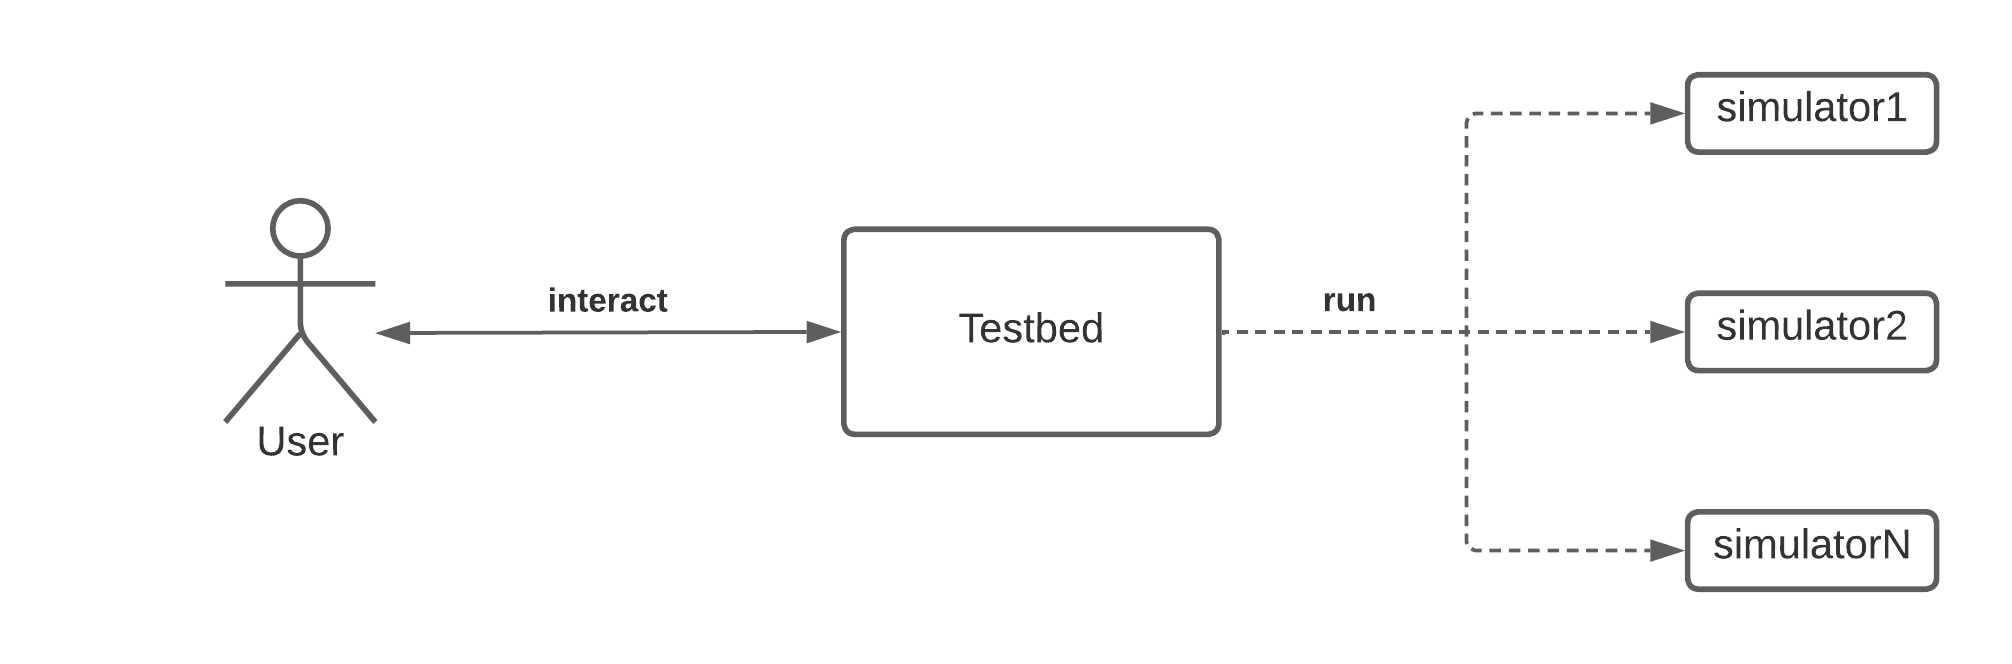
\includegraphics[width=\textwidth]{figures/architecture-high-level.png}
  \caption{Abstract architecture of the testbed}
\end{figure}

The testbed is a framework that sits between the user and the various simulators.
The user specifies which benchmark to run.
The execution of the benchmark is then handled by the testbed, which takes care of running the various scenarios in the respective simulators and collecting the results.

Diving deeper into the architecture, we can see that the testbed is composed of different components, each with a specific role.
The following image shows the architecture of the system.

\begin{figure}[h]
  \centering
  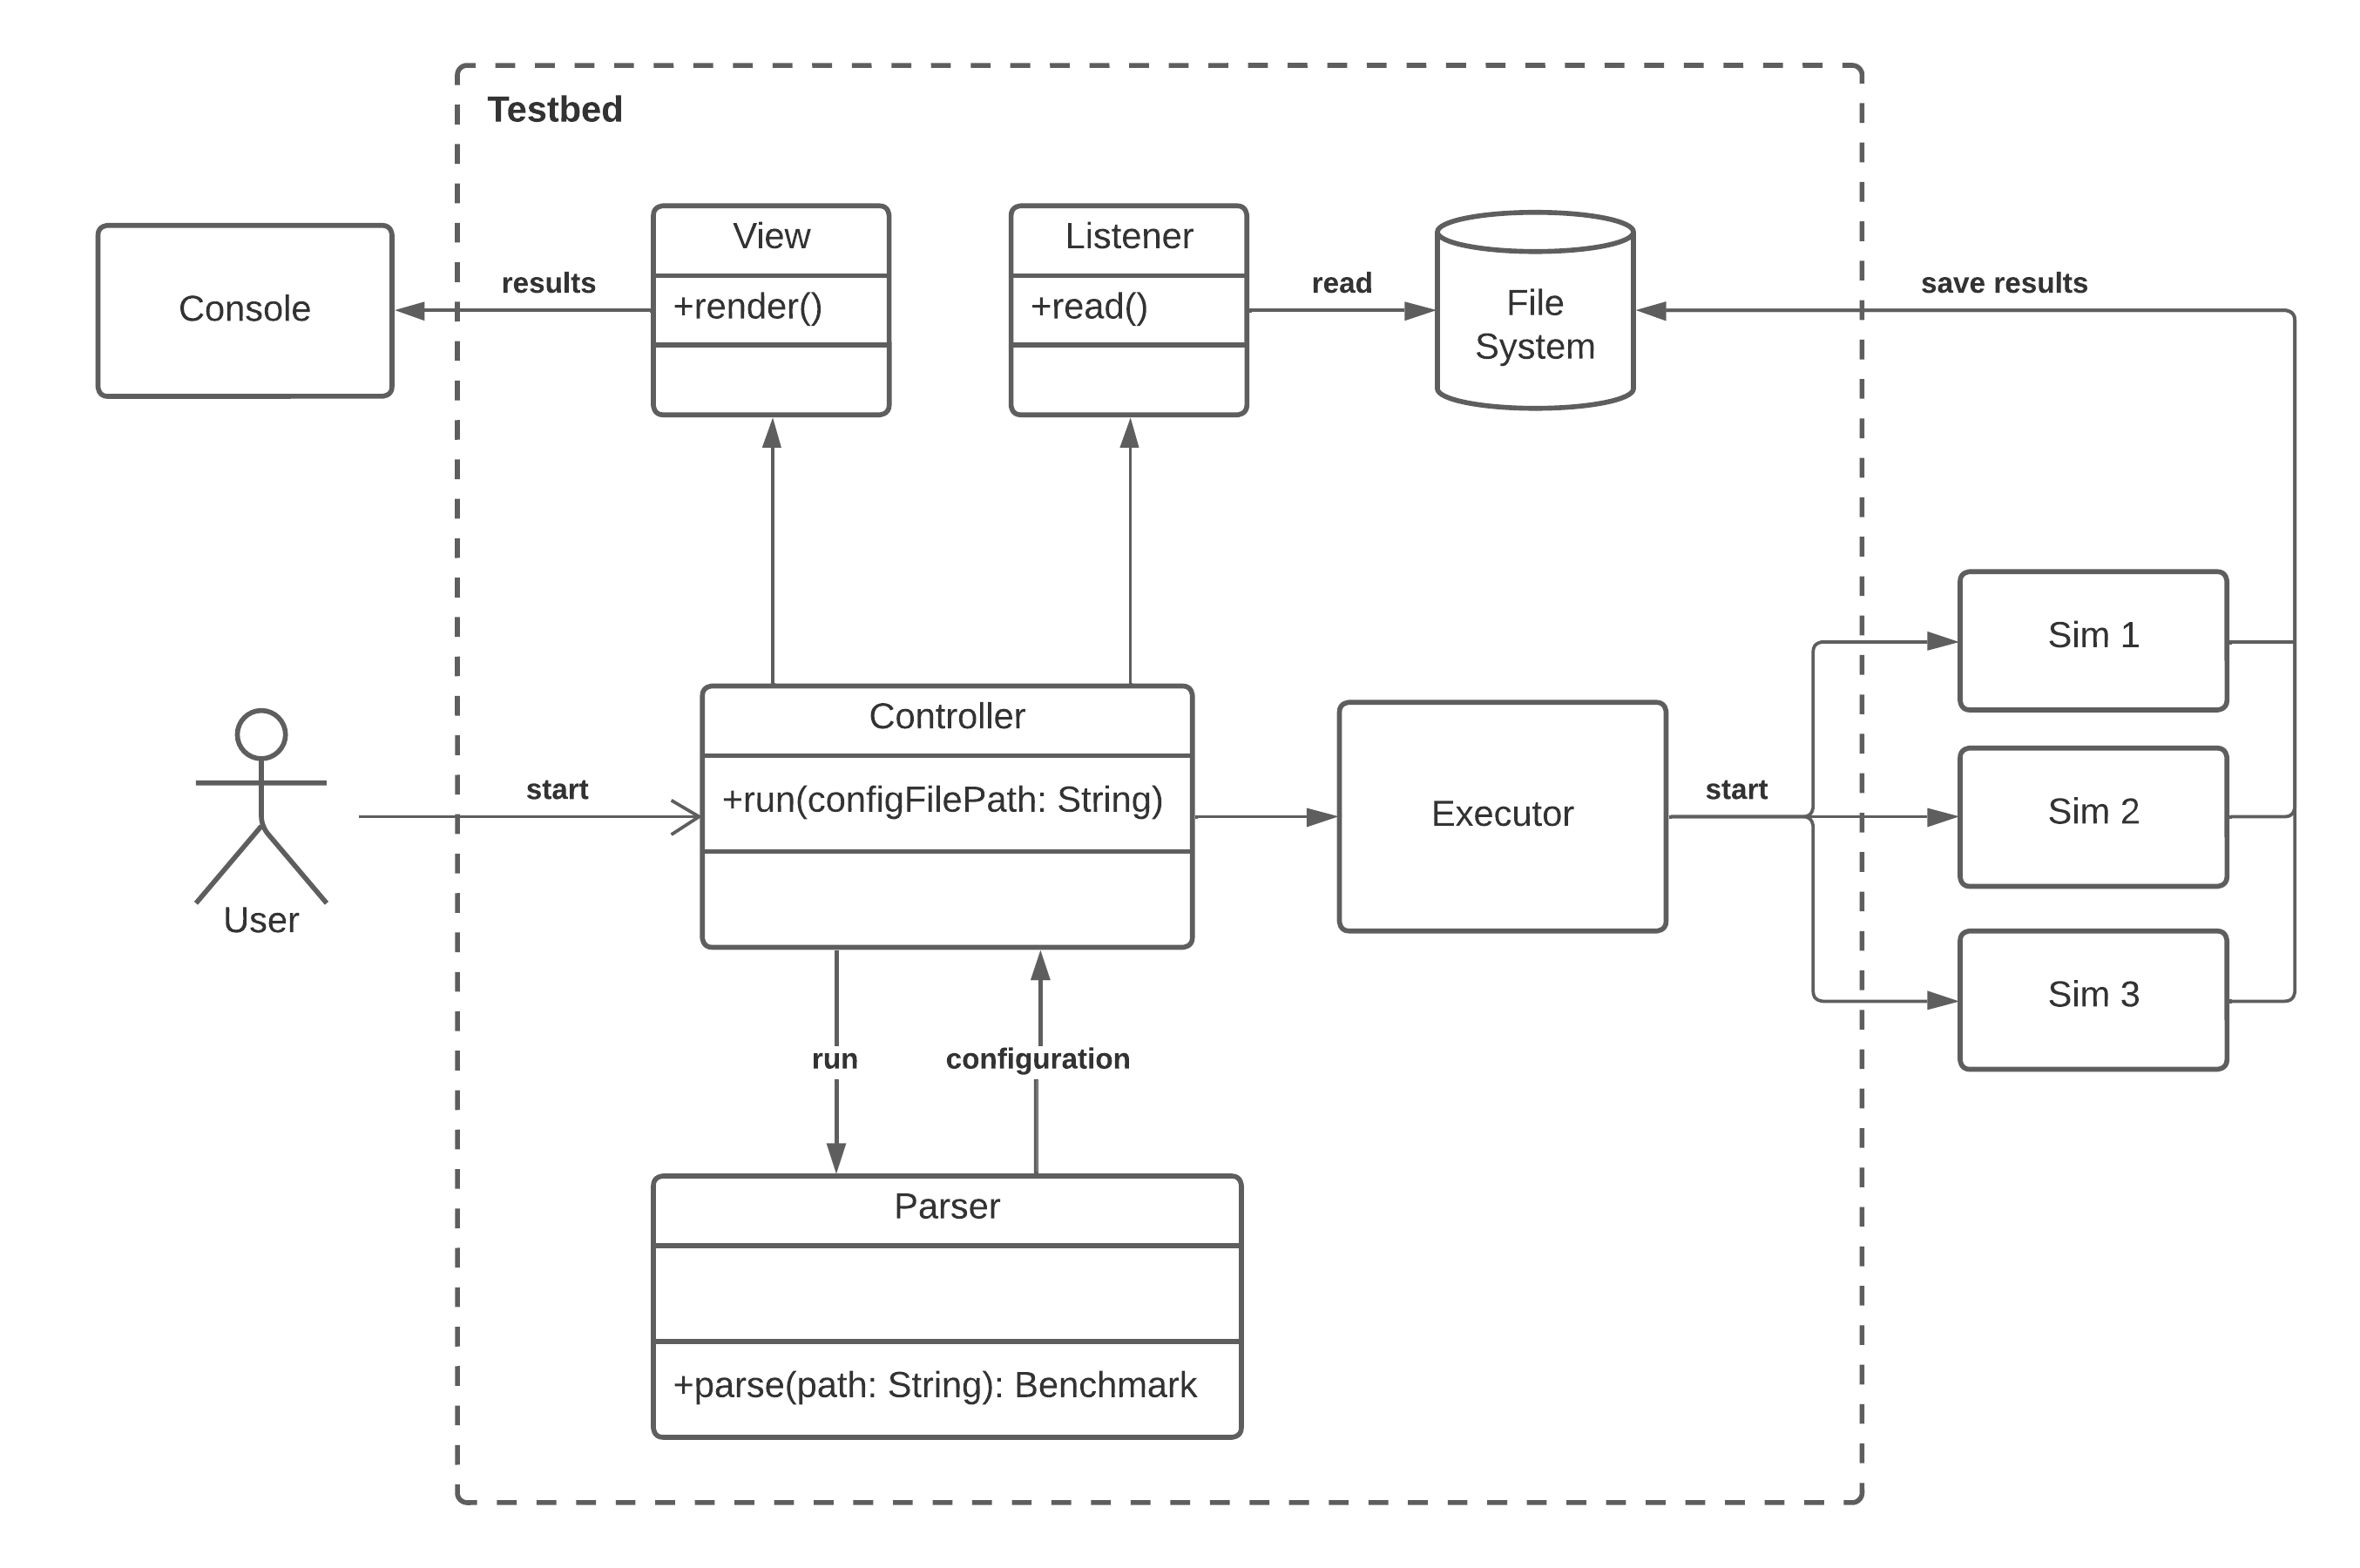
\includegraphics[width=\textwidth]{figures/testbed-architecture.png}
  \caption{Architecture of the system (v0.1)}
  \label{fig:random-image}
\end{figure}

The main component of the Testbed is the controller, which is the entry point of the framework and handles the entire benchmark execution.
The Parser is the component responsible for translating user-written specifications in YAML into a data structure that represents the benchmark model.
If there are manipulations to be made on a configuration file, they will be performed by a Parser component, specific to each simulator, before the actual parsing.
The Executor is responsible for starting the simulator and generating the correct command to invoke the simulator.
For each started simulator, the corresponding Listener is then launched, which reads the simulator's output, cleans the file from unnecessary elements, and saves it in a data structure.
Once the benchmark execution is complete, a post-processing function is applied to the benchmark output to obtain a result of interest, and it is displayed to the user by the View.

To better understand the architecture, it is useful to analyze the execution of a benchmark.

\begin{figure}[h]
  \centering
  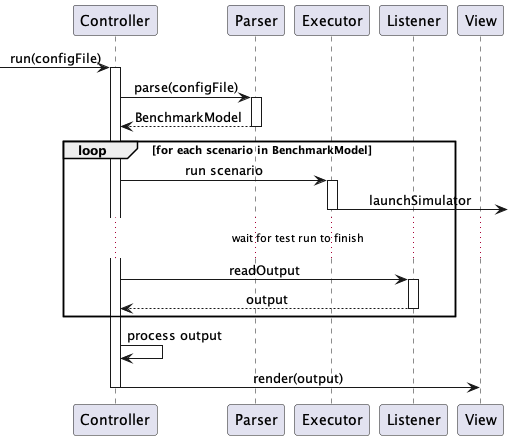
\includegraphics[width=\textwidth]{figures/execution-sequence-diagram.png}
  \caption{Architecture of the system (v0.1)}
  \label{fig:random-image}
\end{figure}

The configuration file is given as input to the controller, which performs some checks on the file's integrity.
Once passed, the controller hands the configuration file to the parser, which, after modifying the file (if necessary), returns to the controller a data structure called BenchmarkModel.
The model contains all the information about the benchmark to be executed.
At this point, each scenario defined by the user must be launched.
The execution is carried out in the order specified by the user.
For each scenario, a command to start the simulator is generated and launched.
The framework then waits for the simulation to finish.
Once it's done, it reads the results returned in output by the simulator and saves them in a data structure.
When the data from all scenarios has been collected, a user-defined transformation is applied to extract results of interest.
These results are finally displayed to the user, either through the console or in a GUI.

\section{Benchmark Configuration}

The design of the input file system is a crucial aspect of the framework.
It should allow the user to define a benchmark simply and intuitively, without limiting the user in any way.
It also needs to be flexible enough to allow the addition of new simulators without breaking the existing structure.

The input file is composed of two main sections: strategy and simulators.

\paragraph*{Strategy}
The strategy section contains generic information about the testbed configuration.
None of these are simulator-specific instructions, but rather general instructions on how the framework will handle the benchmark execution.
At the moment, the only information present in this section is the execution order of the scenarios,
a list that defines the order in which the scenarios will be executed. This is a mandatory parameter.
Other strategy parameters could be added in the future, to enable features such as multi-threaded execution.

\paragraph*{Simulators}
The simulators section contains the configuration of each simulator used for the benchmark.
Each simulator has a name, a path and a list of scenarios.
The name is mandatory and must be written exactly as it appears in the testbed documentation.
The path is optional and is used to specify the path of the simulator executable.
If not specified, the framework will assume that the simulator is in the same directory as the testbed.

\paragraph*{Scenario}
The scenario configuration is more complex, as each simulator has different ways to configure the scenario.
This section contains:
\begin{itemize}
  \item \textbf{name} the name of the scenario. It is mandatory and should match the name in the
  \item \textbf{description} a brief explanation of the scenario. Optional.
  \item \textbf{input} a list of all the input files needed to run the scenario. This parameter is optional to take into account a scenario that does not require any input file.
  \item \textbf{repetitions} the number of times that the scenario should be run. This parameter is optional and defaults to 1.
  \item \textbf{duration} the duration of the simulation. This parameter can be used to overwrite the value present in the simulator-specific configuration file, if the simulator supports it. This parameter is optional.
\end{itemize}

This is an input file example, which will be used to explain the structure of the input file.

\begin{lstlisting}[style=yaml]
strategy:
  executionOrder:
    - Alchemist-sapere-tutorial
    - NetLogo-tutorial
    - Alchemist-protelis-tutorial

simulators:
  - name: NETLOGO
    simulatorPath: "./NetLogo 6.4.0/"
    scenarios:
      - name: NetLogo-tutorial
        description: A tutorial to NetLogo
        input: "../src/main/resources/netlogo/netlogo-tutorial.xml" TODO change to list
        modelPath: "./models/IABM Textbook/chapter 4/Wolf Sheep Simple 5.nlogo"
        repetitions: 3

  - name: Alchemist
    simulatorPath: "./"
    scenarios:
      - name: Alchemist-protelis-tutorial
        description: A tutorial to Alchemist and Protelis incarnation
        input: "src/main/resources/alchemist/protelis-tutorial.yml"
        repetitions: 1
        duration: 10
      - name: Alchemist-sapere-tutorial
        description: A tutorial to Alchemist and Sapere incarnation
        input: "src/main/resources/alchemist/sapere-tutorial.yml"
        repetitions: 1
        duration: 100
\end{lstlisting}

\section{Benchmark Results}

A critical part of the framework design is related to what is presented to the user at the end of the benchmark execution.

We define \emph{output} concepts:
\begin{itemize}
  \item \textbf{Scenario Output} the output of a single scenario. It is a map that associates each metric with its value.
  \item \textbf{Benchmark Output} the output of the entire benchmark. It is a map that associates each scenario with its \emph{Scenario Output}.
\end{itemize}

These concepts represent the data returned at the end of the benchmark execution as generated by the simulator.
This data must be processed in order to extract useful information for the user.

We define \emph{result} concepts, which represent the data the user desires, obtained by processing the benchmark's output.
\begin{itemize}
  \item \textbf{Scenario Result} the result of a single scenario. It contains a description of the result and its value.
  \item \textbf{Benchmark Result} the result of the entire benchmark. It is a list of \emph{Scenario Result}.
\end{itemize}

At this point, it is necessary to define a function to aggregate the data, transforming the benchmark's output to provide useful information to the user.
This function cannot be predefined since, given a benchmark, different users might want to visualize different metrics.
The \emph{processingFunction} is defined as a function that takes as input the \emph{Benchmark Output} and returns the \emph{Benchmark Result}.
The user must implement this function to get the desired result.

\section{Extension}

One of the main goals of this work is to create a flexible system that can be extended to support different simulators.
The architecture was designed considering this characteristic.
Each component of the system has a general behavior, independent of the simulator but incomplete.
This will then be integrated with the specific behavior related to the simulator defined in a subclass.

A user who wants to add support for a new simulator must do the following steps:
\begin{itemize}
  \item Implement the \emph{Executor} interface.
  \item Implement the \emph{Listener} interface.
  \item If some manipulations on the input file are needed, implement the \emph{ConfigFileHandler} interface.
  \item Extend the \emph{SupportedSimulator} enum by adding the new simulator.
  \item Update the \emph{Controller} to take into account the new simulator.
\end{itemize}

%----------------------------------------------------------------------------------------
\chapter{Implementation}
%----------------------------------------------------------------------------------------

In this chapter, we will dive deeper into the implementation of the framework.

\section{Model}

\paragraph*{Benchmark Model}
The benchmark model is the data structure that represents the benchmark to be executed.
It must match the structure of the input file to allow easy parsing.

\begin{figure}[h!]
  \centering
  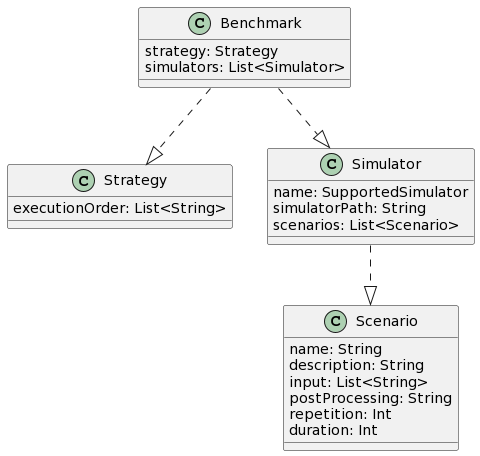
\includegraphics[width=\textwidth]{figures/benchmark-model.png}
  \caption{Benchmark Model}
  \label{fig:benchmark-model}
\end{figure}

Each concept of the model is implemented as a data class in Kotlin, which is a class that only contains data and does not have any functionality.
The \emph{Serializable} annotation is used to allow the model to be serialized and deserialized from YAML.

\begin{lstlisting}[language=Kotlin]
@Serializable
data class BenchmarkModel(
    val strategy: Strategy,
    val simulators: List<Simulator>
)
\end{lstlisting}

\paragraph*{Output and Result}

The concepts of \emph{Scenario Output}, \emph{Benchmark Output} and \emph{Benchmark Result} are implemented as type alias in Kotlin, which is a way to define a new type without creating a new class.
The concept of \emph{Scenario Result} is implemented as a data class.

\begin{lstlisting}[language=Kotlin]
  typealias ScenarioOutput = Map<String, List<Any>>
  typealias BenchmarkOutput = Map<String, ScenarioOutput>
  typealias BenchmarkResult = List<ScenarioResult>

  data class ScenarioResult(
    val description: String,
    val value: List<Any>,
    val visualisationType: VisualisationType,
)
\end{lstlisting}

\section{Technologies}

\subsection*{Framework technologies}

\paragraph*{Kotlin}

Kotlin is a cross-platform, statically typed, general-purpose high-level programming language with type inference.
Kotlin is designed to interoperate fully with Java.
Support for multiplatform programming is one of Kotlin’s key benefits. It reduces time spent writing and maintaining
the same code for different platforms while retaining the flexibility and benefits of native programming.

\paragraph*{YAML}
To provide the user with the ability to write a benchmark configuration file, various options were considered, such as using JSON, YAML, Google Protobuf or even developing a DSL. 
The choice fell on YAML, a human-readable data serialization language. It is a superset of JSON, which means that any valid JSON file is also a valid YAML file.
YAML is commonly used in applications where data needs to be represented in a format that is easy for both humans to read and write, as well as for machines to parse and generate.
In fact, It is used as a configuration language in different projects, such as Kubernetes, Docker, GitHub Actions, and many more.



\subsection*{DevOps technologies}
DevOps engineering is a software development methodology that aims at communication, collaboration and integration among all workers around an IT project. 
This set of techniques responds to interdependencies between software development and relative IT operations, allowing a faster and more efficient organization of software products and services.
The following paragraphs describe which DevOps techniques have been used in the making of the system, focusing on the advantages that each procedure has brought.
\paragraph*{Repository management}
The project was developed following a customized version of Git Flow. 

\begin{figure}[h]
  \centering
  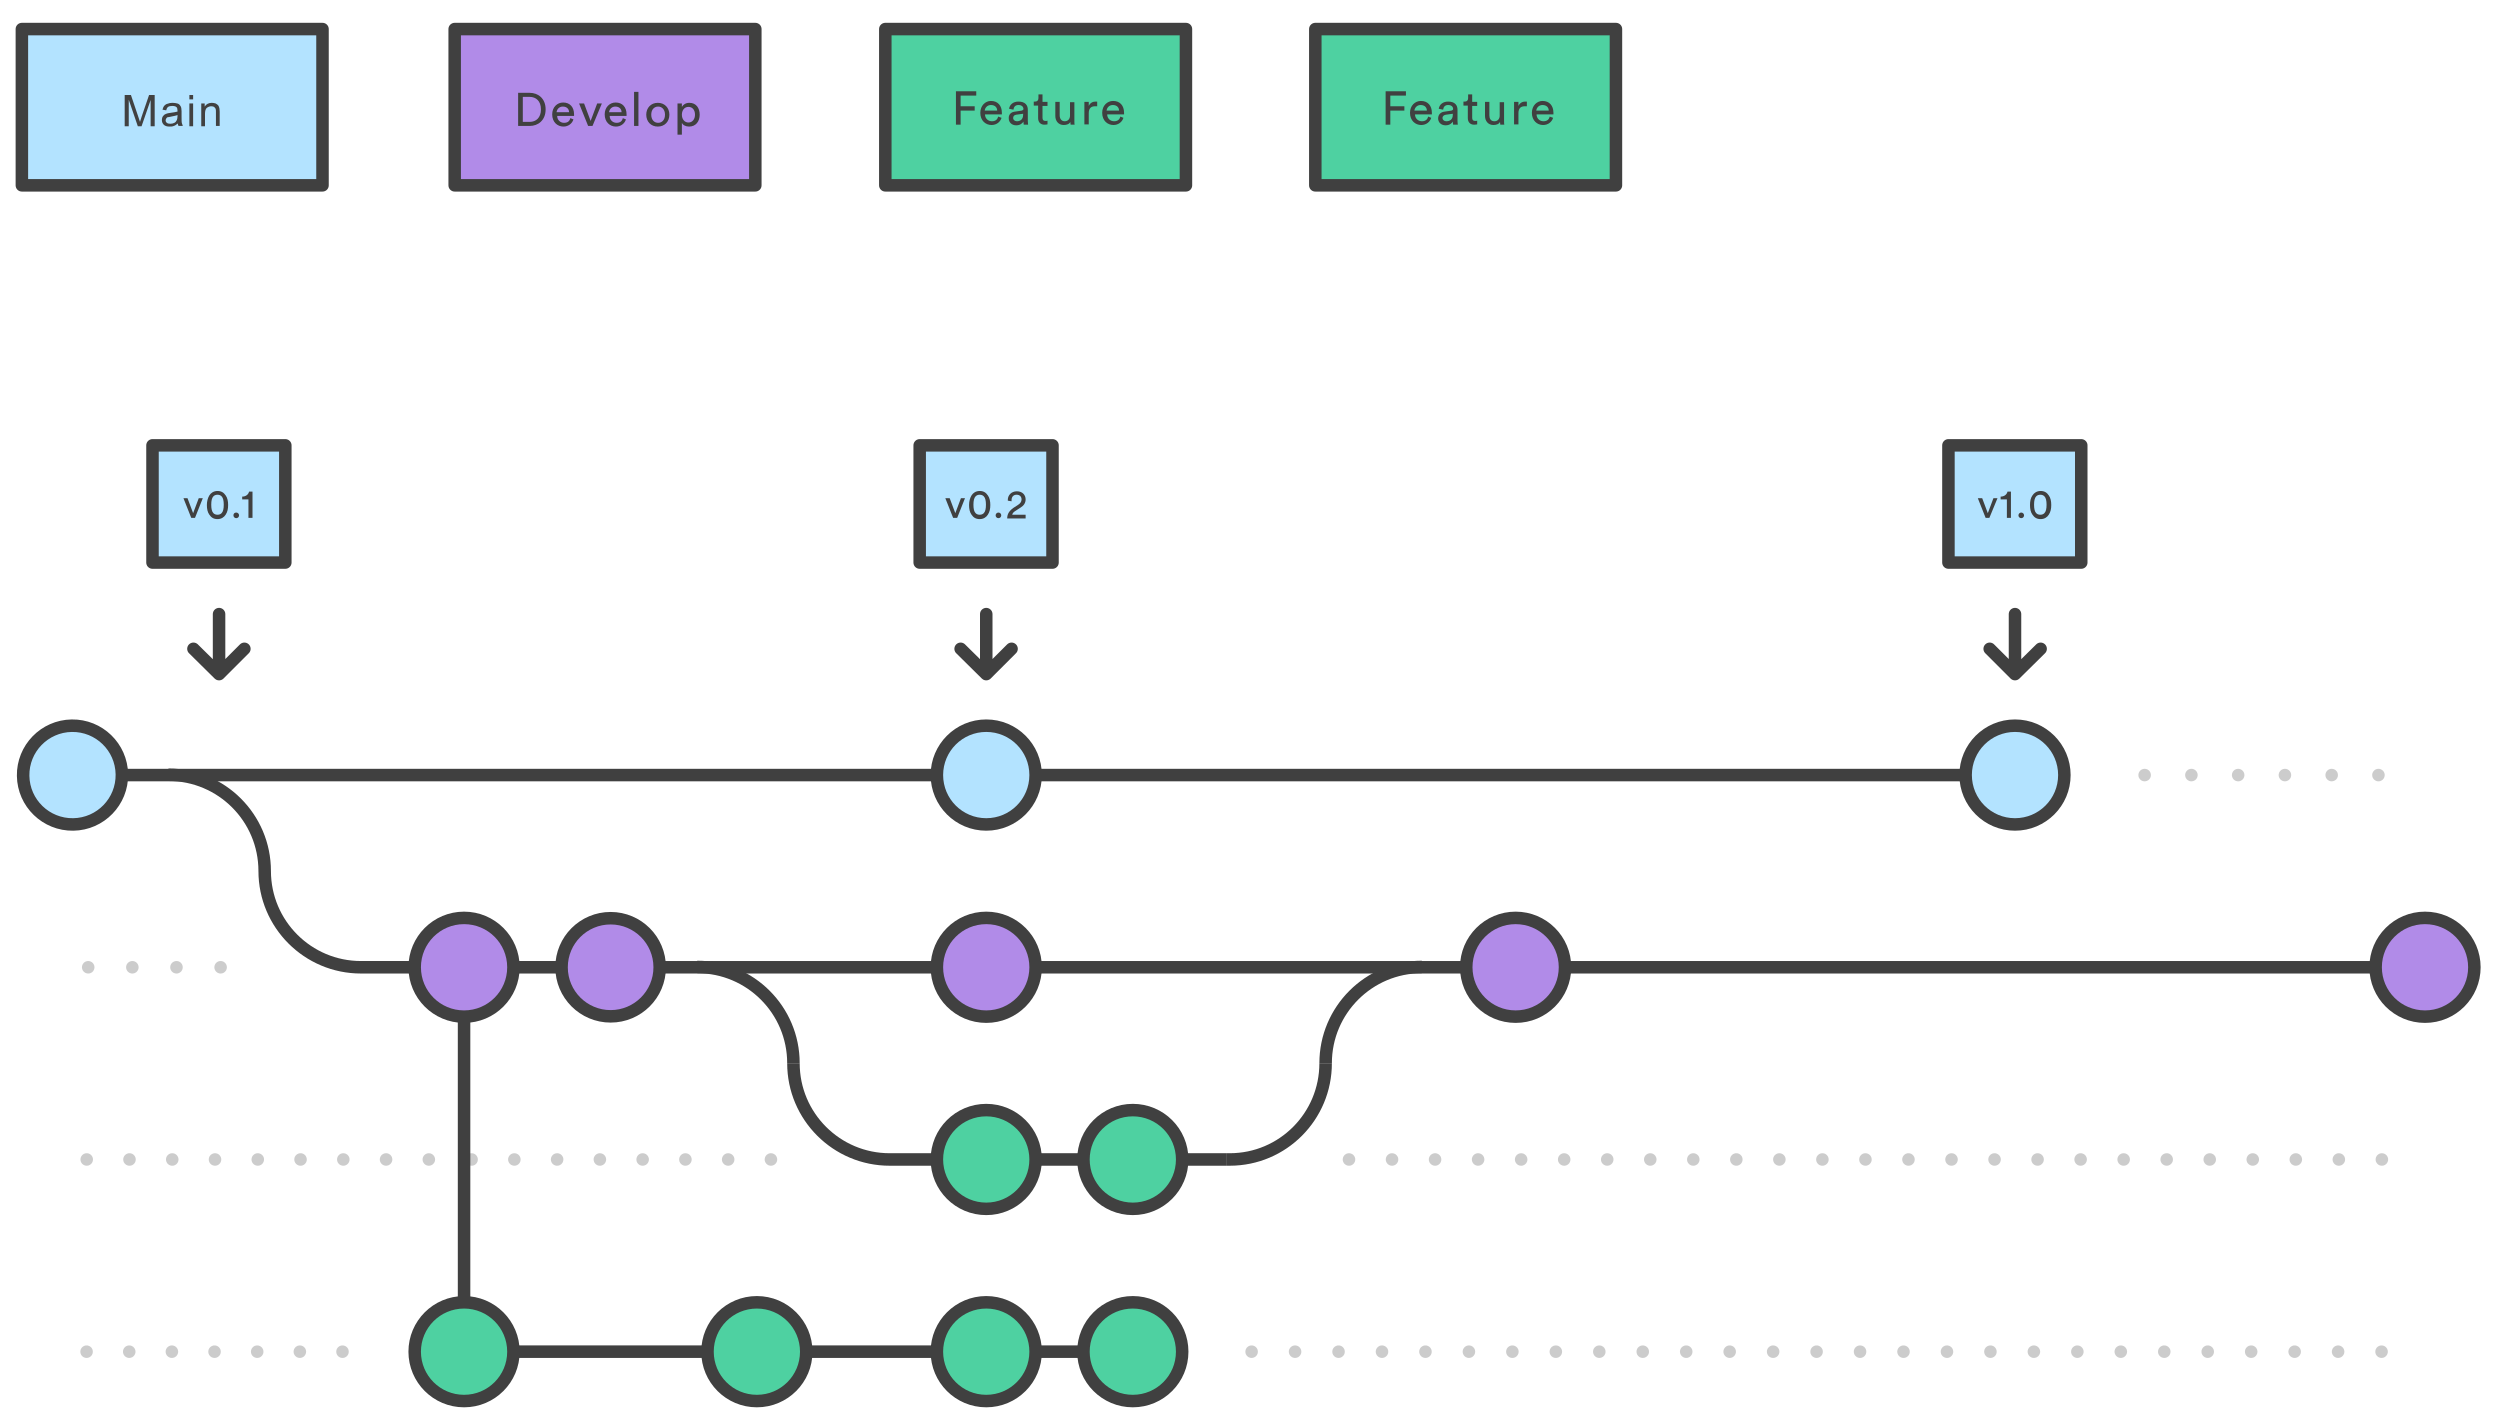
\includegraphics[width=0.8\textwidth]{figures/gitflow.png}
  \caption{Git Flow}
  \label{fig:git-flow}
\end{figure}

The repository consists of a master branch and several feature branches.
The master branch is the development reference: all feature branches originate from it, and at the end of their existence, they are merged into the master branch.
The feature branches are related to the developed features. 
For each feature to be implemented, a feature branch was created, and at the end of the development, a pull request was made to merge the content into the master branch.
All feature branches followed this naming convention: \textit{feature/{feature-name}}

\paragraph*{Build automation}
Build Automation refers to the automation of the build lifecycle of a project, the process from source code to product release and distribution. 
This allows automating operations that were previously done manually, making software deployment more efficient and less error-prone.
In this work, Gradle, one of the most famous and widely used build systems, is used. 
Gradle is primarily used to manage dependencies with external libraries used in the project (e.g., the library for parsing YAML files).
With Gradle, it is possible to define custom tasks, which are essentially atomic operations on the project that have input and output files and can depend on other tasks. 
This functionality has been leveraged to define the task that creates the framework's JAR file, which is then uploaded to GitHub during the release phase.
\begin{lstlisting}
  tasks.withType<ShadowJar> {
    archiveFileName.set("testbed.jar")
    manifest {
        attributes(
            mapOf(
                "Implementation-Title" to "Testbed",
                "Implementation-Version" to rootProject.version.toString(),
                "Main-Class" to "testbed.Testbed",
            ),
        )
    }
}
\end{lstlisting}

\paragraph*{Continuous Integration}
Continuous Integration is a software development practice in which developers regularly merge their code changes into a central repository, after which automated builds and tests are run.
The key goals of continuous integration are to find and address bugs quicker, improve software quality, and reduce the time it takes to validate and release new software updates.
In this work, GitHub Actions is used to automate the process of building, testing, and deploying the framework.
The workflow of a GitHub Action is defined in a YAML file, which is stored in the repository under the path \textit{.github/workflows}.
The following is an example of a GitHub Action that builds the project and runs the tests.

\begin{lstlisting}[language=yaml]
  name: CI/CD Process
on:
  workflow_call:
  workflow_dispatch:

jobs:
  build:
    strategy:
      matrix:
        os: [ windows-2022, macos-12, ubuntu-22.04 ]
    runs-on: ${{ matrix.os }}
    concurrency:
      group: build-${{ github.workflow }}-${{ matrix.os }}-${{ github.event.number || github.ref }}
      cancel-in-progress: true
    steps:
      - name: Checkout
        uses: DanySK/action-checkout@0.2.14
      - name: Test
        run: ./gradlew test
  release:
    concurrency:
      # Only one release job at a time. Strictly sequential.
      group: release-${{ github.workflow }}-${{ github.event.number || github.ref }}
    needs:
      - build
    runs-on: ubuntu-latest
    if: >-
      !github.event.repository.fork
      && (
        github.event_name != 'pull_request'
        || github.event.pull_request.head.repo.full_name == github.repository
      )
    steps:
      - name: Checkout
        uses: actions/checkout@v4.1.1
        with:
          token: ${{ secrets.GH_TOKEN }}
      - name: Find the version of Node from package.json
        id: node-version
        run: echo "version=$(jq -r .engines.node package.json)" >> $GITHUB_OUTPUT
      - name: Install Node
        uses: actions/setup-node@v4.0.2
        with:
          node-version: ${{ steps.node-version.outputs.version }}
      - name: Release
        env:
          GH_TOKEN: ${{ secrets.GH_TOKEN }}
        run: |
          npm install
          npx semantic-release
  success:
    runs-on: ubuntu-22.04
    needs:
      - release
      - build
    if: >-
      always() && (
        contains(join(needs.*.result, ','), 'failure')
        || !contains(join(needs.*.result, ','), 'cancelled')
      )
    steps:
      - name: Verify that there were no failures
        run: ${{ !contains(join(needs.*.result, ','), 'failure') }}
\end{lstlisting}

\paragraph*{Versioning and Releasing}
As for commits, we use Conventional Commit, a convention that provides a set of possible commits, 
each with a different semantic, allowing the definition of the software version number based on the commit history.

The following set of commits is used:
\begin{itemize}
  \item \textbf{Major Release} 
  \begin{itemize}
    \item Any commit terminating \textit{!} causes a \emph{breaking change}
  \end{itemize}

  \item \textbf{Minor Release} 
  \begin{itemize}
    \item Commit type \emph{feat} with any scope.
  \end{itemize}

  \item \textbf{Pathc Release} 
  \begin{itemize}
    \item Commit type \emph{fix} with any scope.
    \item Commit type \emph{docs} with any scope.
    \item Commit type \emph{chore} with scope \textit{core-deps}.
  \end{itemize}

  \item \textbf{No Release} 
  \begin{itemize}
    \item Commit type \emph{test} with any scope.
    \item Commit type \emph{ci} with any scope.
    \item Commit type \emph{chore} with scope \textit{deps}.
    \item Commit type \emph{refactor} with scope \textit{deps}.
  \end{itemize}
\end{itemize}

Thanks to the use of semantic release, it was possible to automate the versioning and releasing of the software. 
Every time a push is made to the master branch, semantic release calculates the version number and creates a release on GitHub, uploading the necessary assets.

The version number is defined in the format \emph{X.Y.Z} where X is a major version, Y the minor version and Z the patch version.
%----------------------------------------------------------------------------------------
\chapter{Validation}
%----------------------------------------------------------------------------------------

\section{Unit Testing}

Unit testing is a software testing method to test individual units or components of software.
In this work, we use it to test the behavior of the various components of the framework.

Given the nature of the work, most components require human judgment to be tested. 
This is the case for the \emph{Executor} and \emph{Listener} components, which are responsible for starting the simulator and reading its output, respectively.
The tests on this component were conducted by repeatedly running the framework with different scenarios and checking the output manually.
The \emph{Parser} component, on the other hand, was tested automatically, to check if the parser correctly translates the input file into the benchmark model.

\begin{lstlisting}[language=kotlin]
  class ParserTest : FreeSpec({
    "The parser" - {
        val parser: Parser = ParserImpl()
        "should parse a partial input file" {
            // ARRANGE
            val expectedBenchmark = simpleBenchmarkBuilder()
            // ACT
            val benchmark = parser.parse("src/test/resources/SimpleBenchmark.yml")
            // ASSERT
            assert(benchmark == expectedBenchmark)
        }
        "should parse a full input file" {
            val expectedBenchmark = fullBenchmarkBuilder()
            val benchmark = parser.parse("src/test/resources/FullBenchmark.yml")
            assert(benchmark == expectedBenchmark)
        }
        "should fail to parse a wrong file" {
            assertThrows<InvalidPropertyValueException> {
                parser.parse("src/test/resources/WrongBenchmark.yml")
            }
        }
    }
})
\end{lstlisting}

\section{Integration Testing}

Integration testing is a software testing method to test the behavior of the various components of the software when integrated together.
In this work, we use it to test the behavior of the simulators supported by the framework.

Checking if a simulator is running a scenario in the right way is not an easy task to do automatically, as it requires human judgment.
Therefore the integration tests are performed manually.

\paragraph*{NetLogo}
NetLogo was tested by running one of the bundled models, the Wolf Sheep Predation model.

The first time, the simulation was launched through the framework in headless mode, without a graphical interface. 
Several logs were added to monitor the benchmark execution, and everything went as expected: 
the parser generated the benchmark model, which was used by the controller and executor to launch the simulation. 
At the end of the simulation, an output file containing the expected information was generated. 
This CSV file was then transformed into a data structure within the framework containing the results.

The second execution was launched again through the framework, but this time with the graphical interface activated. 
The same steps as before were observed, with the addition of the simulation being visually displayed.

Comparing the two executions and conducting further ones, no differences were noticed. 
We can therefore say that NetLogo has been integrated correctly into the framework.

\begin{figure}
  \centering
  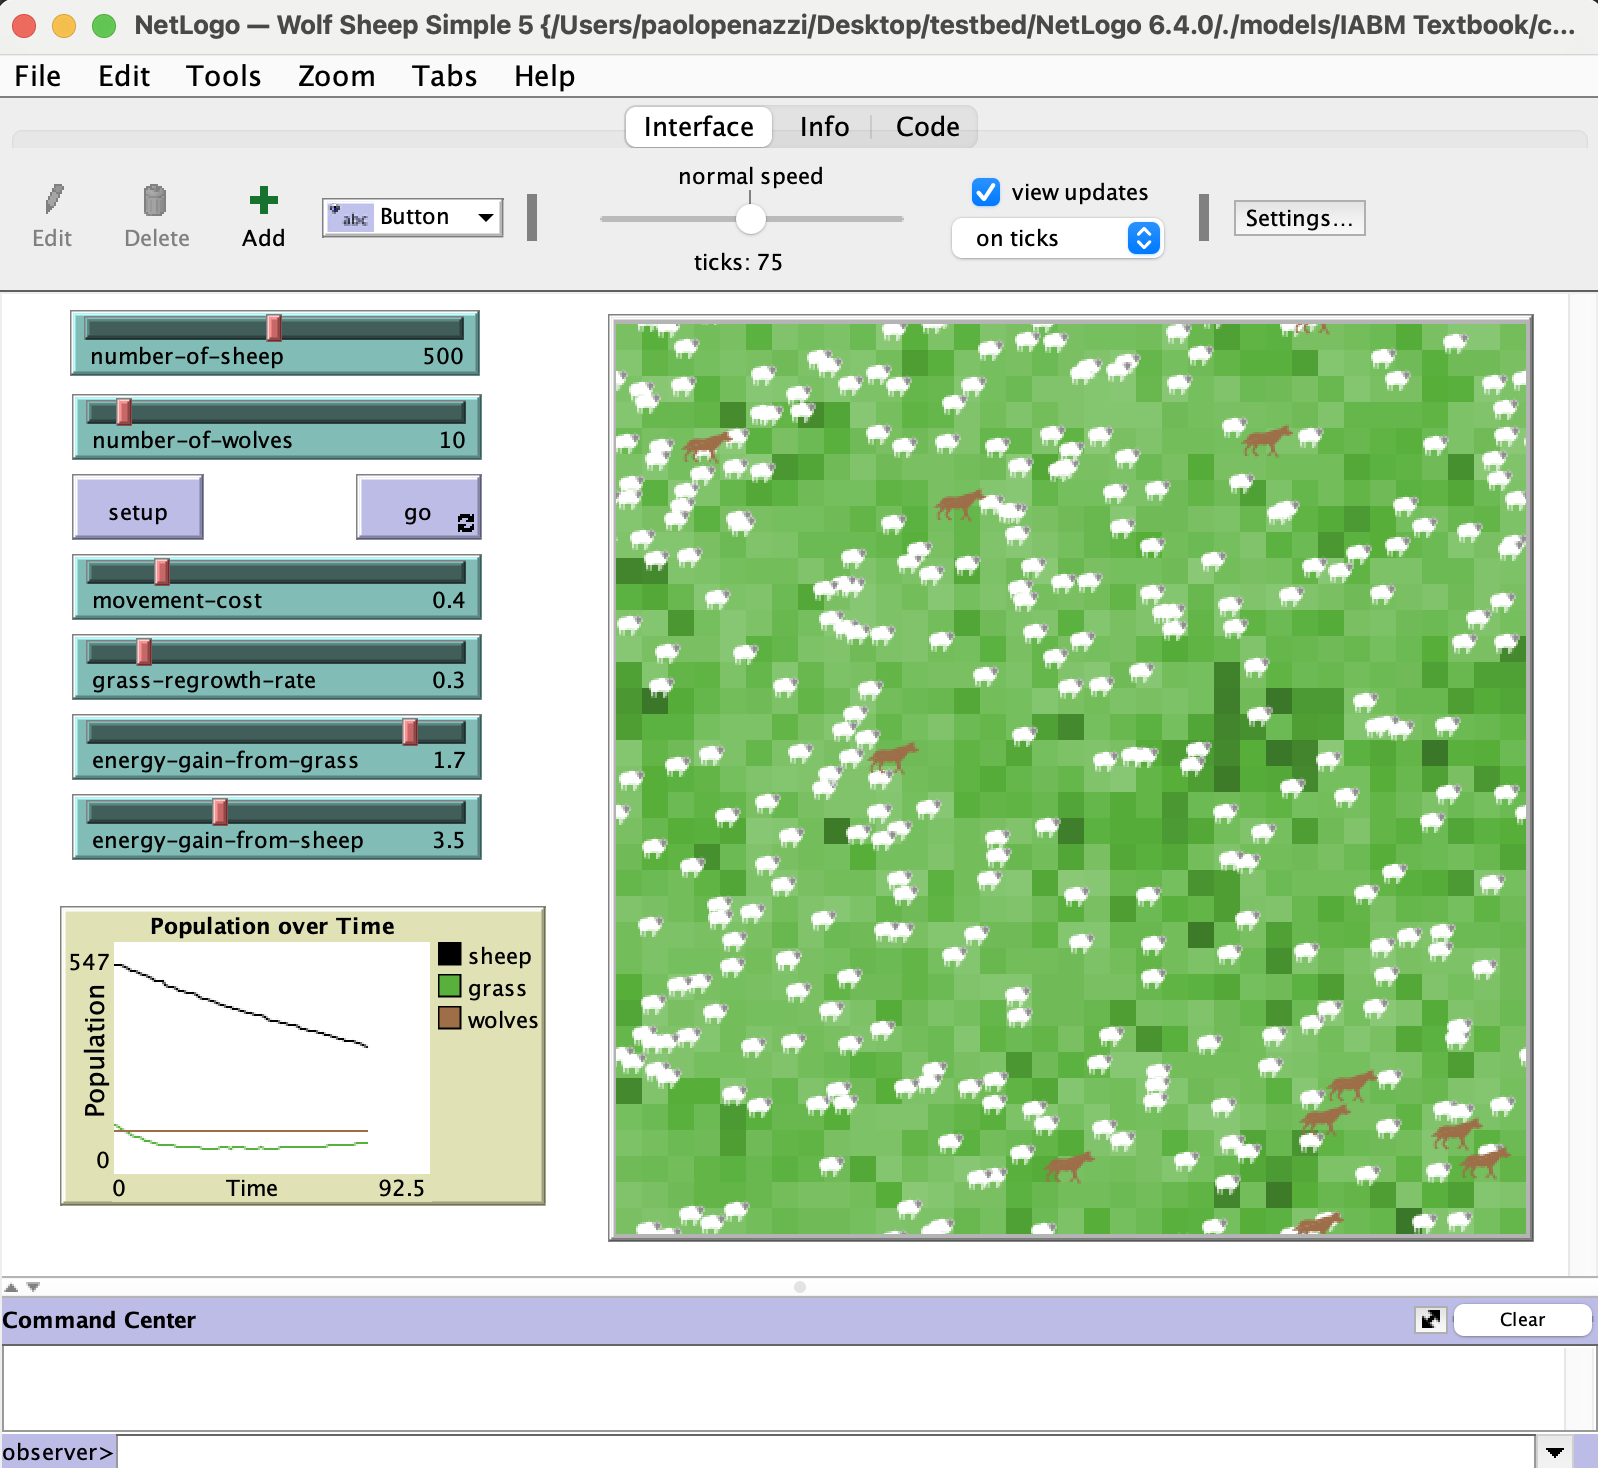
\includegraphics[width=0.8\textwidth]{figures/netlogo-sim.png}
  \caption{NetLogo simulation launched by the framework}
\end{figure}

\paragraph*{Alchemist}
The same process was applied to test the integration with the Alchemist simulator. 
In this case, even more tests were conducted to verify the support for two Alchemist incarnations, namely Protelis and SAPERE.

Again, both executions with a graphical interface, where the correct progress of the simulation could be verified, 
and headless executions yielded the same results.



\section{Acceptance Testing}
Acceptance testing is a software testing method to test the behavior of the software from the user's perspective.






%----------------------------------------------------------------------------------------
\chapter{Conclusion and Future Work}
%----------------------------------------------------------------------------------------

%----------------------------------------------------------------------------------------
% BIBLIOGRAPHY
%----------------------------------------------------------------------------------------

\backmatter

%\nocite{*} % comment this to only show the referenced entries from the .bib file

\bibliographystyle{plain}
\bibliography{bibliography}

\end{document}
